%
\pdfoutput=1
\pdfminorversion=5 % necessary for EES
%
%\documentclass[12pt,number,sort&compress,preprint,review]{elsarticle}
\documentclass[smallextended,referee]{svjour3}

\smartqed

\journalname{}
% better printing of numbers
\usepackage[utf8]{inputenc}
\usepackage[T1]{fontenc}
\usepackage[english]{babel}
\usepackage{graphicx}
\usepackage{latexsym, amsmath, amssymb}


\begin{document}


\title{Modeling atmospheric chemistry using Cantera reactor networks.}

\titlerunning{Modeling atmospheric chemistry using Cantera reactor networks.}

\author{Anthony S.~Walker}

\institute{A.~Walker \at
           School of Mechanical, Industrial, and Manufacturing Engineering, Oregon State University, Corvallis, OR, USA \\
           \email{kyle.niemeyer@oregonstate.edu}
}

\date{Received: date / Accepted: date}
\def\pyplume{\texttt{PyPlume}}
\def\SCALE{0.7}

\maketitle 

% We present recent work on the swept rule, a domain decomposition strategy for explicit solutions to partial differential equations, on heterogeneous, distributed architectures, in particular those commonly found on compute clusters containing GPGPU accelerators.
\begin{abstract}
\texttt{PyPlume} is a software developed for the purpose of atmospheric modeling. The software focuses on building complicated reactor networks to more practically simulate atmospheric chemistry. 
\end{abstract}


\section{Introduction}
Chemistry plays an important role in many aspects of today's society such as transportation, healthcare, energy production, and environmental safety and protection. As we continue to relay on the burning of matter to extract energy, it is important to understand the impact that our actions have on society and our planet. Is all the fuel we burn detrimental to our health in the long term? To what degree can we safely continue our way of life? Are we destroying other forms of life on the planet as well with out behavior? The list of important questions goes on and answering them is no minor feat.

Answering these questions definitively requires scientific study to develop and model the lifespan and behavior of products from burning matter. Small scale phenomena can be analyzed experimentally to determine constituents and potential impacts. However, how do you experimentally model wildfire that burns hundreds of thousands of acres with an immense variety of different fuels both living and dead? How do you model the burning of a jet fuel which has thousands of different chemical species to track? How do you follow the products from both scenarios throughout the atmosphere across the world? The answer would seem to be computational modeling, but it has it's limitations as well. First and foremost, modeling such complicated phenomena requires a lot of computing resources. The models can be simplified to use less resources but at the cost of accuracy.

Aircraft contrails are a large contributor to radiative forcing

\section{Motivation}


\section{Methods}

\pyplume{} was built with Cantera\cite{cantera} at it's core. The goal was to create a versatile \texttt{Python} tool that can generate complicated exhaust models with a reactor network approach. While complicated models are currently constrained by expense, I am working towards implemented methods to drastically accelerate the solution process and reduce this expense. This package was created with the intention of using these methods on a particular application such as a more rigorous study of aircraft exhaust. \pyplume{} focuses on the exhaust portion of the system but also includes a reservoir-combustor network to generate the input conditions and, an atmospheric reservoir for mass entrainment into the exhaust network. The general idea is shown in Figure~\ref{fig:general}.

\begin{figure}
    \centering
    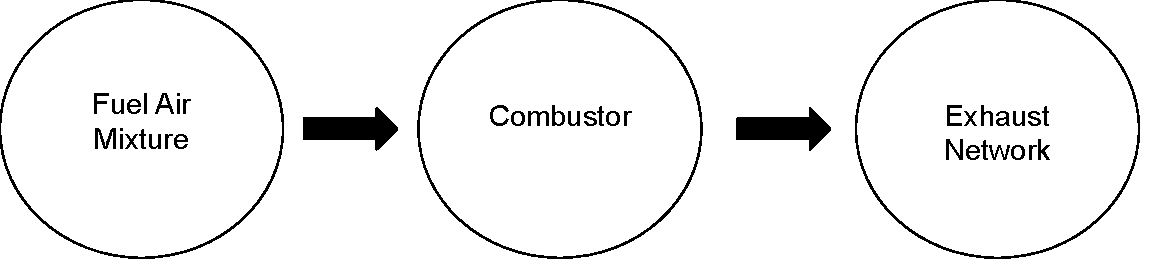
\includegraphics[scale=\SCALE]{examples/report/figs/general.pdf}
    \caption{General concept for modeling exhaust networks in pyplume.}
    \label{fig:general}
\end{figure}

So, how do we produce a more in-depth study with a set of well-stirred ideal gas reactors? The main idea that I had was the ability to relax the well mixed nature of well-stirred reactors. This can be achieved with multiple connected reactors, entrainment, and mass conservation. \pyplume{} uses an adjacency matrix approach to creating and connecting the exhaust reactor network which makes this possible, e.g., mass entrainment into an outer reactor will provide a different concentration than inner reactors. The second idea was to use larger mechanisms that include more of elementary reactions. This is also possible with the package because the mechanism can be independently specified for every reactor if desired.

These ideas led to the development of three models within \pyplume: \texttt{simple}, \texttt{linear}, and \texttt{grid}. The simple model was used primarily in developing and testing and is shown in Figure~\ref{fig:simple}. 

\begin{figure}[htp!]
    \centering
    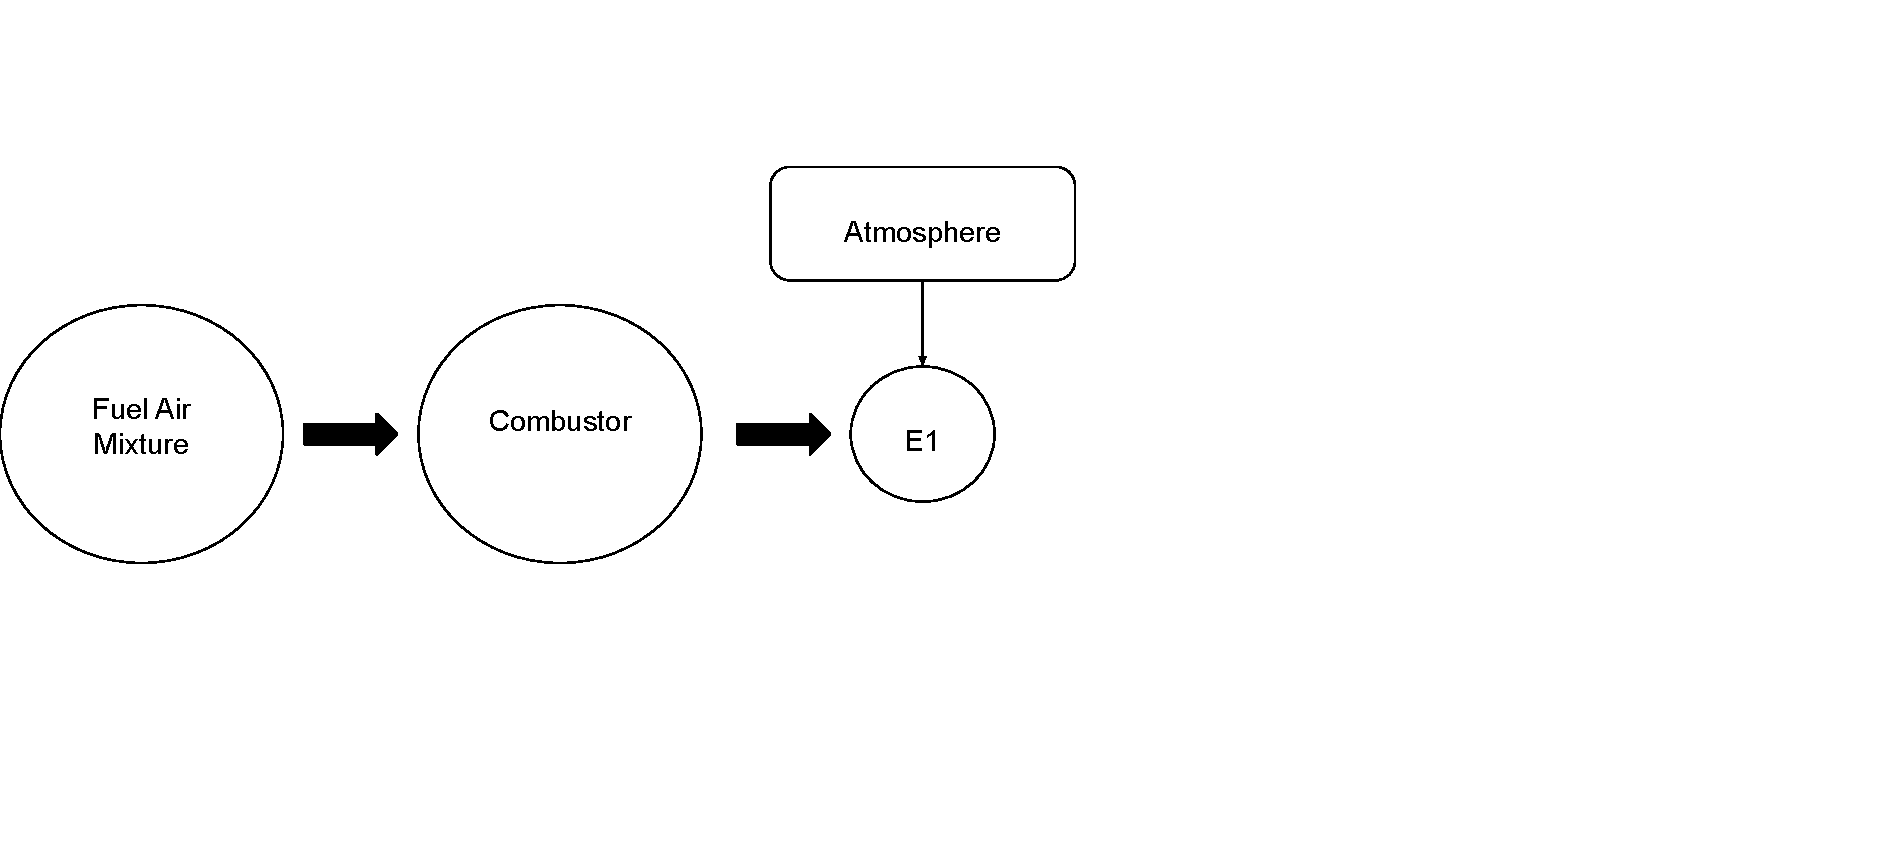
\includegraphics[scale=\SCALE,trim=1cm 5cm 1cm 4cm]{examples/report/figs/simple.pdf}
    \caption{Simple model for testing and developing.}
    \label{fig:simple}
\end{figure}

The \texttt{grid} and \texttt{linear} models were developed as different takes on achieving a less well mixed system but they have yet to be formally tested and verified to this end. These models aside, \pyplume{} can be used to develop other models by providing an adjacency matrix to the software. I suspect this will be the the most useful for my application. For example, to produce the \texttt{linear}, and \texttt{grid} model shown in Figures~\ref{fig:linear} and \ref{fig:grid}, the adjacency matrices would respectively be 
\setcounter{MaxMatrixCols}{12}
\renewcommand*{\arraystretch}{0.5}
\begin{equation*}
    \begin{bmatrix}
     0 & 1 & 1 & 0 & 0 & 0 & 0 & 0 & 0 & 0 & 0 \\
     0 & 0 & 0 & 1 & 1 & 1 & 0 & 0 & 0 & 0 & 0 \\
     0 & 0 & 0 & 1 & 1 & 1 & 0 & 0 & 0 & 0 & 0 \\
     0 & 0 & 0 & 0 & 0 & 0 & 1 & 1 & 1 & 1 & 0 \\
     0 & 0 & 0 & 0 & 0 & 0 & 1 & 1 & 1 & 1 & 0 \\
     0 & 0 & 0 & 0 & 0 & 0 & 1 & 1 & 1 & 1 & 0 \\
     0 & 0 & 0 & 0 & 0 & 0 & 0 & 0 & 0 & 0 & 0 \\ 
     0 & 0 & 0 & 0 & 0 & 0 & 0 & 0 & 0 & 0 & 0 \\ 
     0 & 0 & 0 & 0 & 0 & 0 & 0 & 0 & 0 & 0 & 0 \\ 
     0 & 0 & 0 & 0 & 0 & 0 & 0 & 0 & 0 & 0 & 0 \\ 
     1 & 1 & 1 & 1 & 0 & 1 & 1 & 0 & 0 & 1 & 0 
    \end{bmatrix}\quad and\quad
    \begin{bmatrix}
     0 & 1 & 1 & 1 & 0 & 0 & 0 & 0 & 0 & 0 & 0 \\
     0 & 0 & 0 & 0 & 1 & 0 & 0 & 0 & 0 & 0 & 0 \\
     0 & 0 & 0 & 0 & 0 & 1 & 0 & 0 & 0 & 0 & 0 \\
     0 & 0 & 0 & 0 & 0 & 0 & 1 & 0 & 0 & 0 & 0 \\
     0 & 0 & 0 & 0 & 0 & 0 & 0 & 1 & 0 & 0 & 0 \\
     0 & 0 & 0 & 0 & 0 & 0 & 0 & 0 & 1 & 0 & 0 \\
     0 & 0 & 0 & 0 & 0 & 0 & 0 & 0 & 0 & 1 & 0 \\
     0 & 0 & 0 & 0 & 0 & 0 & 0 & 0 & 0 & 0 & 0 \\
     0 & 0 & 0 & 0 & 0 & 0 & 0 & 0 & 0 & 0 & 0 \\
     0 & 0 & 0 & 0 & 0 & 0 & 0 & 0 & 0 & 0 & 0 \\
     1 & 1 & 0 & 1 & 1 & 0 & 1 & 1 & 0 & 1 & 0 
 \end{bmatrix}.
\end{equation*}

\begin{figure}
    \centering
    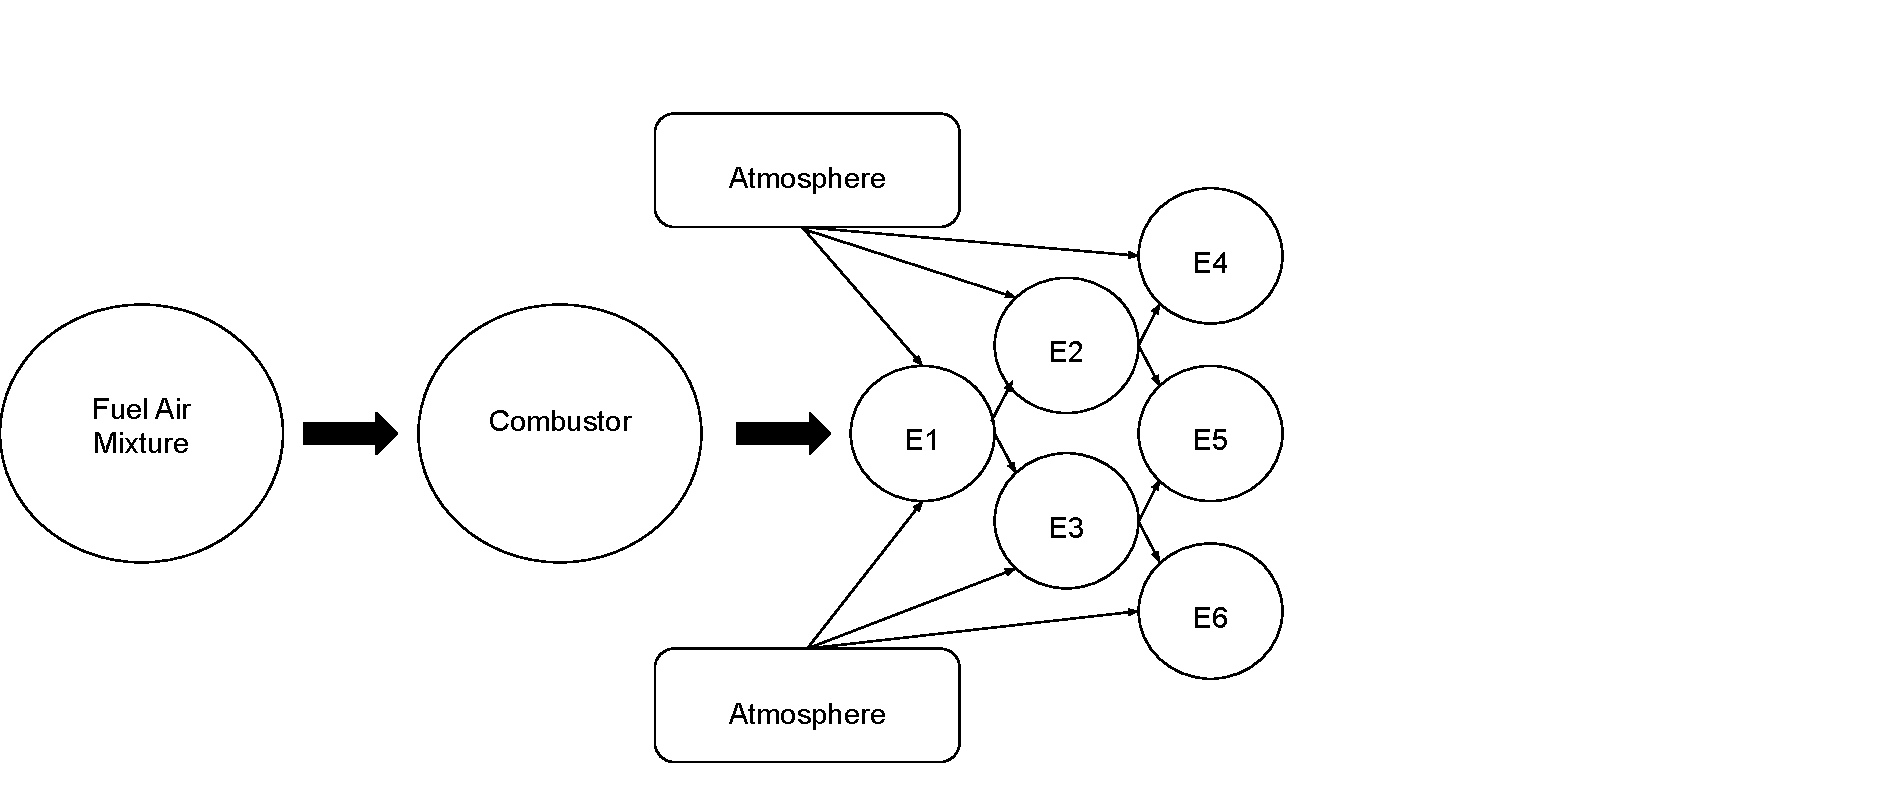
\includegraphics[scale=\SCALE,trim=1cm 1cm 1cm 1cm]{examples/report/figs/linear.pdf}
    \caption{Linear model for developing a less well mixed system.}
    \label{fig:linear}
\end{figure}

\begin{figure}
    \centering
    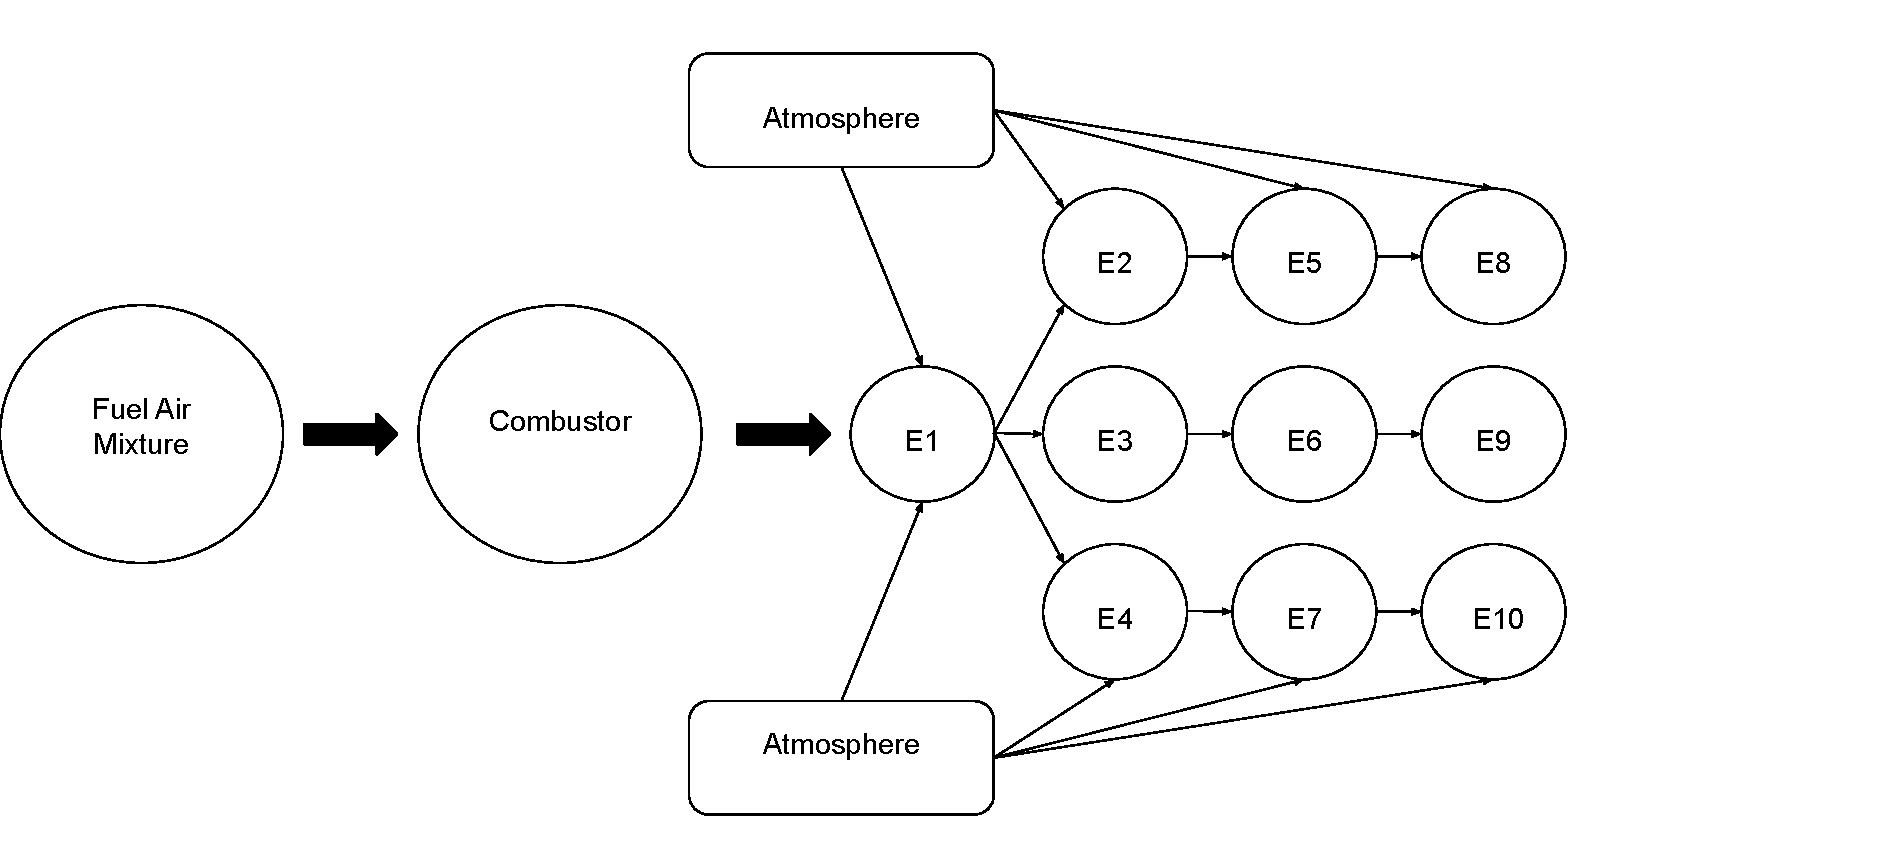
\includegraphics[scale=\SCALE,trim=1cm 1cm 1cm 1cm]{examples/report/figs/grid.pdf}
    \caption{Grid model for developing a less well mixed system.}
    \label{fig:grid}
\end{figure}


\section{Results}

\section{Conclusions}

\begin{acknowledgements}

\end{acknowledgements}

\appendix


\bibliographystyle{plainurl}
\bibliography{references}

\end{document}
